\documentclass[12pt,a4paper,twoside]{book}
\usepackage{graphicx}
\usepackage{setspace}	%double spacing for text, single for captions, footnotes, etc.
%\usepackage{hypernat} 	%substitut de cite que permet fer hyperlinks
\usepackage{natbib}		% substituye a 'hypernat' que funciona en Windows.
\usepackage[spanish]{babel}
\usepackage[utf8]{inputenc}
\usepackage{color}
\usepackage{hhline} 		% extended styles for tables
\usepackage{multirow}
\usepackage{subfigure}
\usepackage{acronym}
\usepackage{hyperref}
\usepackage{amsmath,amsmath,amssymb} 
\usepackage{fancyhdr}
\usepackage{epsfig, amsmath}
\usepackage{algorithm}
\usepackage{algorithmic}

% general settings
\hypersetup{
	linktocpage=true,
	colorlinks=true,
	linkcolor=blue,
	citecolor=blue,
}
\definecolor{Hgray}{gray}{0.6}

\newenvironment{definition}[1][Definition]{\begin{trivlist}
\item[\hskip \labelsep {\bfseries #1}]}{\end{trivlist}}

\setlength{\topmargin}{0cm}
\setlength{\textheight}{23cm}
\setlength{\textwidth}{17cm}
\setlength{\oddsidemargin}{0cm}
\setlength{\evensidemargin}{0cm}
\setlength{\headheight}{1cm}

% indica que las 'sub-sub-sections' sean numeradas y aparezcan en el indice
\setcounter{secnumdepth}{3}
\setcounter{tocdepth}{2}

% settings for code
\renewcommand{\algorithmicrequire}{\textbf{Entrada: }}
\renewcommand{\algorithmicensure}{\textbf{Salida: }}

%%%%%%%%%%%%
% DOCUMENT %
%%%%%%%%%%%%
\begin{document}

% portada
\newpage
\thispagestyle{empty}

\baselineskip 2em

%\vspace*{1cm}

\centerline{
\includegraphics[width=0.6\textwidth]{images/UOC-logo}}
\begin{center}
\textsc{Universitat Oberta de Catalunya (UOC) \\
 Máster Universitario en Ciencia de Datos (\textit{Data Science})\\}

%\centerline {\pic{UOC}{4cm}}

\vspace*{1.5cm}

\textsc{\Large TRABAJO FINAL DE MÁSTER}

\vspace*{0.5cm}

\textsc{\large Área: Informática, Multimedia y Telecomunicación}


%\textbf{\Huge VirtualTechLab Model: }

\vspace*{2.0cm}

\textbf{\Large Predicción de Panel Attrition con Machine Learning: El caso de la Encuesta Financiera de las Familias}

\textbf{\large }

\vspace{2.5cm}
\baselineskip 1em

\baselineskip 2em
-----------------------------------------------------------------------------\\
Autor:      Carlos Luis Gento de Celis\\
Tutor:      Jordi Escayola Mansilla\\
Profesor:   Ismael Benito Altamirano\\
-----------------------------------------------------------------------------\\
\vspace*{1.5cm}
Madrid, \today

\end{center}

\newpage
\pagestyle{empty}
\hfill

\newpage
% abstract
\pagenumbering{roman} 
\setcounter{page}{1} 
\pagestyle{plain}

%%%%%%%%%%%%%%%%
%%% CREDITOS %%%
%%%%%%%%%%%%%%%%
\chapter*{Créditos/Copyright}

\vspace{1cm}

\begin{figure}[ht]
    \centering
	
\includegraphics[scale=1]{images/license.png}
\end{figure}

Esta obra está sujeta a una licencia de Reconocimiento -  NoComercial - SinObraDerivada

\href{https://creativecommons.org/licenses/by-nc-nd/3.0/es/}{3.0 España de CreativeCommons}.

%%%%%%%%%%%%%
%%% FICHA %%%
%%%%%%%%%%%%%
\chapter*{FICHA DEL TRABAJO FINAL}

\begin{table}[ht]
	\centering{}
	\renewcommand{\arraystretch}{2}
	\begin{tabular}{r | p{10cm}}
		\hline
		Título del trabajo: & Predecir panel attrition con Machine Learning: Un análisis con la Encuesta Financiera de las Familias\\
		\hline
        Nombre del autor: & Carlos Luis Gento de Celis\\
		\hline
        Nombre del colaborador/a docente: & Jordi Escayola Mansilla\\
		\hline
        Nombre del PRA: & Antonio Lozano Bagén\\
		\hline
        Fecha de entrega (mm/aaaa): & 10/2023\\
		\hline
        Titulación o programa: & Máster Universitario en Ciencia de Datos\\
		\hline
        Área del Trabajo Final: & Informática, Multimedia y Telecomunicación\\
		\hline
        Idioma del trabajo: & Español\\
		\hline
        Palabras clave & predictive models, machine learning, panel attrition\\
		\hline
	\end{tabular}
\end{table}

%%%%%%%%%%%%%%%%
%%% RESUMEN  %%%
%%%%%%%%%%%%%%%%

\chapter*{Resumen}
\addcontentsline{toc}{chapter}{Resumen}

\onehalfspacing

La Encuesta Financiera de las Familias (EFF) es una encuesta bienal cuyo objetivo es recoger información sobre la situación económico-financiera de los hogares que residen en España, y su evolución a lo largo del tiempo. Para ello, los hogares seleccionados pueden participar en hasta cuatro olas consecutivas de la encuesta. Sin embargo, hay hogares que abandonan el estudio antes de tiempo. Aunque estos abandonos no interrumpan el estudio, sí podrían afectar a sus resultados si el número de abandonos es demasiado grande, o si se concentra en colectivos específicos de la población. Es importante analizar las causas de estos abandonos y desarrollar herramientas que puedan evitarlos.

Este documento, en primer lugar, analiza las características de los hogares que participaron en la Encuesta Financiera de las Familias (EFF) en sus ediciones de 2017 y 2020, y si participaron en las olas de 2020 y de 2022. A continuación, plantea una serie modelos de predicción basados en métodos de Machine Learning y evalúa su capacidad para predecir si un hogar abandonará la EFF en 2020 o en 2022. Finalmente, interpreta los resultados el modelo que mejor ha funcionado.

\vspace{1.5cm}

\textbf{Palabras clave}: predictive models, panel attrition, machine learning, household surveys

\chapter*{Abstract}
\addcontentsline{toc}{chapter}{Abstract}

\onehalfspacing

The Spanish Survey of Household Finances (EFF) is a biennial survey whose goal is to collect information about the economical and financial situation of households in Spain, and its evolution through time. To do so, selected households may take part in up to four consecutive waves of this survey. However, some households cease their participation prematurely. Although withdrawals do not interrupt the research study, they might affect its results if the number of withdrawals is too high, or if it is more likely to happen for certain groups of people. It is important to analyse the causes of this phenomenon and develop tools to prevent it.

Firstly, this paper analyses the characteristics of households that responded to the EFF in its editions of 2017 and 2020, and their participation during the 2020 or 2022 waves. Next, a series of predictive models based on machine learning methods are considered and evaluated for the exercise of predicting panel attrition in the EFF. Finally, it interprets the results of the most successful model.

\vspace{1.5cm}

\textbf{Key words}: predictive models, panel attrition, machine learning, longitudinal surveys, household surveys
\newpage

\pagestyle{fancy}
\renewcommand{\chaptermark}[1]{ \markboth{#1}{}}
\renewcommand{\sectionmark}[1]{\markright{ \thesection.\ #1}}
\lhead[\fancyplain{}{\bfseries\thepage}]{\fancyplain{}{\bfseries\rightmark}}
\rhead[\fancyplain{}{\bfseries\leftmark}]{\fancyplain{}{\bfseries\thepage}}
\cfoot{}

% indice
\cleardoublepage
\phantomsection
\addcontentsline{toc}{chapter}{Índice}
\tableofcontents

\thispagestyle{empty}

\pagenumbering{arabic}

\pagestyle{fancy}
\renewcommand{\chaptermark}[1]{ \markboth{#1}{}}
\renewcommand{\sectionmark}[1]{\markright{ \thesection.\ #1}}
\lhead[\fancyplain{}{\bfseries\thepage}]{\fancyplain{}{\bfseries\rightmark}}
\rhead[\fancyplain{}{\bfseries\leftmark}]{\fancyplain{}{\bfseries\thepage}}
\cfoot{}

\onehalfspacing

% capitulos del documento
\chapter{Introducción}
\label{chapter:introduccion}

Los estudios longitudinales son proyectos de investigación en los que se hace un seguimiento a un grupo de unidades muestrales (personas, hogares...) a lo largo de un período de tiempo. En el ámbito de las ciencias sociales, la recolección de datos de muchos de estos estudios se realiza mediante el uso de encuestas, de tal manera que las mismas personas responden a las preguntas del mismo cuestionario de manera repetida durante un tiempo, que pueden ser semanas, meses o incluso años. Esto da lugar a las llamadas encuestas longitudinales o encuestas panel. La dimensión temporal de estas encuestas las convierten en una herramienta muy útil para poder analizar relaciones causales, ya que permiten observar cambios en opiniones, comportamientos o estados de los mismos panelistas a lo largo del tiempo. Sin embargo, la calidad de esos análisis depende de la cooperación exitosa y continuada de dichos panelistas durante las sucesivas ediciones u olas de la encuesta. El abandono prematuro y acumulado en el tiempo de participantes en un panel se conoce como \textbf{Panel Attrition} (\cite{watson2009identifying}).

\cite{lynn2018tackling} destaca que el Panel Attrition presenta dos principales problemas. Por un lado, si la tasa de abandonos es alta, el tamaño de la muestra se reducirá drásticamente en pocas olas, lo que provocará que la precisión de los estimadores de la encuesta sea muy baja, y además limitará o incluso imposibilitará el análisis de subgrupos dentro de la muestra. Por otro lado, si el Panel Attrition no es aleatorio y los panelistas que abandonan la encuesta son sistemáticamente diferentes a los que se mantienen, existe el riesgo de introducir un sesgo de no-respuesta en los estimadores de la encuesta.

Tradicionalmente, los métodos utilizados para mitigar los efectos del Panel Attrition se han centrado en el impacto estadístico que provoca, principalmente con el uso de métodos de imputación múltiple (\cite{rubin1987multiple}), la reponderación de pesos muestrales (\cite{groves2009survey}) e introduciendo muestras de refresco para sustituir a las unidades muestrales perdidas (\cite{hirano1998combining}). Pero en las últimas décadas ha aumentado el interés por tratarlo durante los procesos de creación y recolección de datos, lo que ha llevado a la extensión del uso de los llamados diseños adaptativos y reactivos (adaptative and responsive designs, \cite{tourangeau2017adaptive}). La idea detrás de estos diseños se fundamenta en utilizar toda la información que se genera durante la elaboración de encuestas (respuestas al cuestionario, paradata u observaciones de los entrevistadores) para diseñar implementaciones informadas cuyo objetivo sea mejorar la calidad de los datos, reducir los costes, o ambos. En este sentido, las encuestas longitudinales ofrecen una gran oportunidad para estos diseños porque contienen mucha información tanto de los trabajos de campo que se estén desarrollando, como los que se realizaron en olas anteriores. Por ejemplo, se ha utilizado información sobre intentos de contacto en olas pasadas para revisar la estrategia de incentivos para hogares a los que cuesta volver a entrevistar (\cite{mcgonagle2022effects}) o para optimizar las estrategias de contacto en las ediciones siguientes (\cite{kreuter2015note}).

Dentro de este contexto de los diseños adaptativos y reactivos, en las últimas décadas se ha desarrollado el uso algoritmos de Machine Learning en la metodología de encuestas, especialmente para predecir Panel Attrition (\cite{buskirk2018introduction}). Por ejemplo, en \cite{beste2023case} utilizan información de ediciones pasadas de una encuesta a hogares en Alemania para entrenar varios modelos basados en algoritmos de Machine Learning para identificar hogares panelistas con una baja probabilidad de volver a participar en la siguiente edición. Posteriormente, utilizan el mejor de esos modelos para predecir cuáles hogares panelistas de una nueva edición tenían menor probabilidad de colaborar de nuevo, y usan esas predicciones para crear un diseño experimental enfocado en esos hogares.

El objetivo de este Trabajo de Fin de Máster es adaptar la implementación de Machine Learning vista en \cite{beste2023case} para predecir la participación de los hogares panel al caso de estudio de la Encuesta Financiera de las Familias (EFF). La EFF es una encuesta a hogares representativa de los hogares que residen en España, y es creada por el Banco de España. La idea central del ejercicio de predicción consiste en utilizar información de hogares en olas pasadas de la EFF para predecir una variable binaria de participación o no participación en la ola siguiente. Para ello, se entrenan cuatro modelos basados en algoritmos de Machine Learning y se compara su rendimiento con un modelo de referencia utilizado tradicionalmente en análisis de Panel Attrition, que en este caso es una Regresión Logística o Logit. En este proyecto, para el entrenamiento de los modelos se utiliza información sobre hogares que han participado en las olas 4, 5, 6 y 7 de la EFF (que se corresponden con los años 2011, 2014, 2017 y 2020), y a continuación se utilizan dichos modelos para predecir la participación de los hogares panel elegibles para la ola 8 (que se corresponde con el año 2022).

Los seis capítulos restantes de este documento se organizan de la siguiente manera. En el siguiente capítulo se exponen los objetivos, la planificación del proyecto y las motivaciones personales para realizarlo. En el tercer capítulo se hace una revisión del estado del arte para este estudio, en el que se describe cuáles son las causas del Panel Attrition, cómo se están utilizado algoritmos de Machine Learning para predecirlo, y finalmente se presenta la Encuesta Financiera de las Familias (EFF). En el cuarto capítulo se describe la metodología utilizada en el análisis exploratorio de datos y en el ejercicio de entrenamiento, validación y test de los modelos de predicción de Panel Attrition. En el quinto capítulo se presentan los datos de la EFF y se realizan una descripción de las etapas de producción de la EFF, y un análisis exploratorio de los datos. En el sexto capítulo se muestran y comentan los resultados del entrenamiento y la evaluación de los modelos de predicción, y se analiza la importancia de las variables utilizadas en uno de los modelos de predicción para explicar el Panel Attrition. Finalmente, en el último capítulo se exponen las conclusiones y reflexiones sobre el proyecto y cuáles pueden ser las líneas de trabajo para el futuro.
\chapter{Objetivos del proyecto, planificación y motivación personal}
\label{chapter:objetivos}
\section{Objetivos del proyecto}

Este proyecto se contextualiza dentro del marco de la metodología de encuestas. En concreto, se centra en las encuestas longitudinales a hogares, y dentro de ese campo pone el foco en la predicción de la participación de los hogares en olas posteriores a su primera colaboración. La encuesta elegida para el proyecto es la Encuesta Financiera de las Familias (EFF), una encuesta de referencia para investigaciones sobre finanzas de los hogares.

El \textbf{objetivo principal} de este proyecto es desarrollar un modelo de predicción basado en métodos de machine learning que ayude a predecir si un hogar que ha participado en al menos una ola de la EFF volverá a hacerlo en olas posteriores.

Para poder desarrollar ese modelo, es necesario completar una serie de \textbf{objetivos secundarios}. Estos objetivos se agruparán en 5 fases:

\begin{enumerate}[noitemsep]
    \item Hacer una revisión del estado del arte sobre el Panel Attrition y las metodologías de Machine Learning aplicadas a su predicción.
    \item Recolección de datos. Preferentemente, obtener un conjunto de datos que contenga:
    \begin{enumerate}
        \item Las respuestas de los hogares al cuestionario de la EFF.
        \item Paradata sobre el proceso de creación de la encuesta.
        \item Características de los entrevistadores.
    \end{enumerate}
    \item Análisis exploratorio de los datos. Identificar patrones dentro de los datos que puedan estar relacionados con el panel attrition.
    \item Preprocesar los datos para entrenar modelos de machine learning.
    \item Modelado y evaluación de modelos de predicción basados en métodos de machine learning.
    \item Interpretación del mejor modelo y redacción de conclusiones.
\end{enumerate}

\section{Planificación del proyecto}

La planificación de este proyecto se va a dividir en 5 fases. La asignación temporal a cada una de ellas se ha realizado de acuerdo a la estructura de contenidos del Plan Docente y al calendario de la asginatura.

\begin{enumerate}[noitemsep]
    \item Fase 1: Contiene la definición del proyecto y la planificación del TFM. Abarca las dos primeras semanas del proyecto, del 27 de septiembre al 10 de octubre.
    \item Fase 2: Contiene las tareas de la revisión de la literatura y la caracterización del panel attrition de la EFF. Abarcará desde el 11 de octubre al 23 de octubre.
    \item Fase 3: Contiene las tareas de recolección de datos, análisis exploratorio de dichos datos, preprocesamiento para entrenar los modelos de machine learning, modelado y evaluación de los modelos de predicción, y la interpretación de los modelos y la redacción de conclusiones. Esta fase es la más duradera y abarcará desde el 17 de octubre al 19 de diciembre.
    \item Fase 4: En esta fase se procederá a la redacción de la memoria del TFM y la preparación de una presentación audiovisual sobre el proyecto. Abarcará desde el 20 de diciembre al 18 de enero.
    \item Fase 5: En esta fase final se procederá a la defensa del TFM. Esa etapa abarcará desde el 22 de enero hasta el 4 de febrero.
\end{enumerate}

 En la figura \ref{fig:gantt} puede observarse la distribución temporal y el tiempo dedicado a cada tarea en un diagrama de Gantt.


\begin{figure}
	\centering
	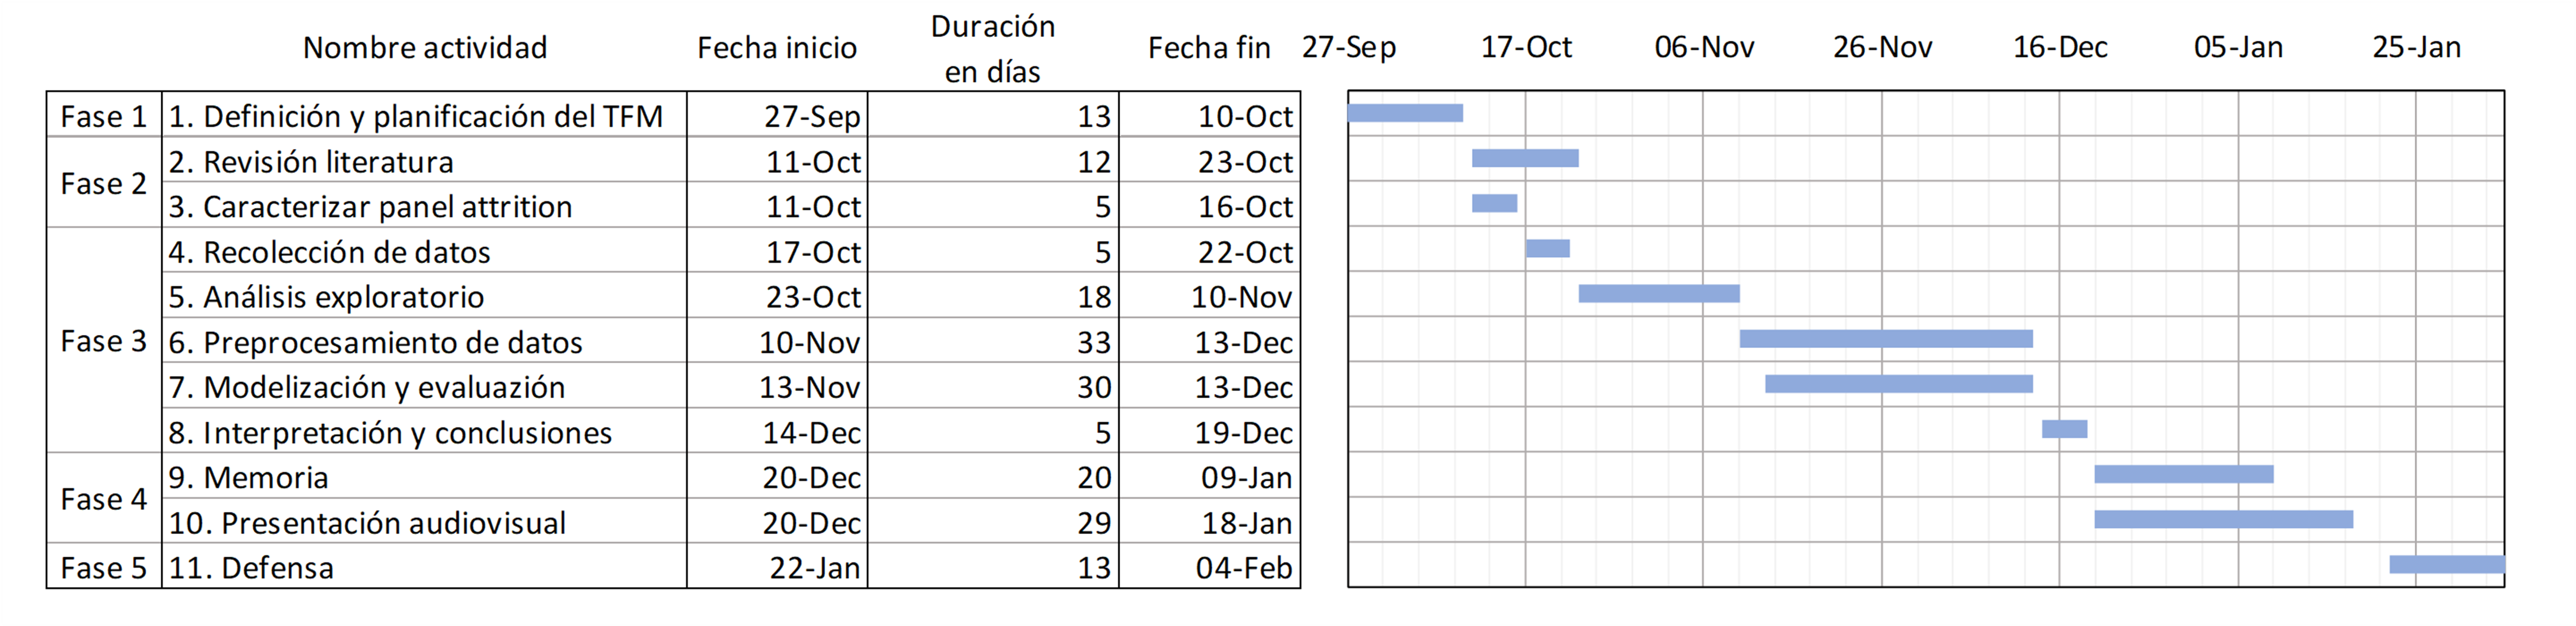
\includegraphics[width=1\textwidth]{figs/Gantt_diagram.png}
	\caption{Planificación de las actividades del TFM}
	\label{fig:gantt}
\end{figure}

\section{Motivación personal}

Trabajo para el Banco de España, y formo parte del equipo que elabora la Encuesta Financiera de las Familias (EFF) desde principios de 2015. He participado en la elaboración de sus cuatro últimas ediciones (EFF2014, EFF2017, EFF2020 y EFF2022) y con los años ha crecido mi interés por la metodología de encuestas y el potencial que tienen para recoger información sobre fenónemos que de otra manera serían difíciles de captar. La EFF es una fuente de información de referencia en el campo de las finanzas de los hogares y eso hace más importante realizar trabajos y esfuerzos para garantizar e incluso mejorar la calidad de sus datos. En ese sentido, la gran cantidad de paradatos que se generan durante cada ola ofrecen muchas oportunidades para aprender sobre todo el proceso y encontrar maneras de mejorarlo.

Por otro lado, en los últimos años ha aumentado cantidad de datos que se generan durante la encuesta y también su variedad, tomando espacecial relevancia los audios de las entrevistas y los comentarios de texto escritos por los entrevistadores, que se han convertido en herramientas fundamentales de los procesos de revisión de calidad de los datos. Los métodos y las herramientas desarrolladas en el campo de la ciencia de datos abren un mundo de posibilidades para poder analizar y explotar toda esa información.

Finalmente, sobre el Panel Attrition, considero que la etapa más importante de la elaboración de la EFF es el trabajo de campo. En ella se contacta a los hogares, se les convence para participar en la encuesta y se realizan las entrevistas. Marca el devenir las siguientes etapas, y también el nivel de calidad de los datos. Por esa razón, es importante conseguir la colaboración de los hogares. Especialmente la de los hogares panel, ya que representan una proporción importante de la muestra, y no convercerles puede llegar a ser muy costoso. Y es un área que en la EFF no se ha podido explorar hasta. Es una gran oportunidad para aprender.
\input{3_datos_metodologia}
\chapter{Resultados y posibles próximos pasos}
\label{chapter:resultados}

Este capítulo está compuesto por dos secciones. En la primera sección se muestran varios resultados y patrones observados durante el análisis explotarorio de los datos de la EFF, y cómo algunos de ellos han influido en la toma de decisiones con respecto a las variables que finalmente han entrado en los modelos. Finalmente, en la segunda sección se comentan los resultados de la evaluación de los diferentes modelos de machine learning utilizados durante este estudio.

Antes de empezar con los resultados, es importante destacar la gran cantidad de variables e información que se recoge en la EFF. En el Cuadro 4.1 se recoge el número de registros y variables disponibles en cada uno de los ficheros utilizados, después de seleccionar sólo a los hogares elegibles para la EFF2020 y a los entrevistadores que participaron en la EFF2017. El número de hogares elegibles para la EFF2020 es de 5.938, el número de entrevistadores en 69 y el número de pantallas que se vieron en el CAPI durante todas las entrevistas es 2.578.926\footnote{Los registros del fichero de paradata son las pantallas del ordenador con las que interactúa el entrevistador durante la entrevista. Suele haber una pregunta por pantalla, y cuando se responde, se pasa a la siguiente pantalla. Cuantas más preguntas, más pantallas se ven.}.

\begin{table}[h]
    \centering{}
    \begin{tabular}{ | l | c | c |}
    \hline
    Nombre del fichero & Registros & Variables \\ \hline
    Fichero de trabajo & 5.938 & 6.103 \\
    Fichero de datos imputados  & 5.938 & 659 \\
    Fichero de recontactos  & 5.938 & 4 \\
    Fichero de contactos  & 5.938 & 636 \\
    Censo de entrevistadores  & 69 & 56 \\
    Fichero paradata  & 2.578.926 & 13 \\
    \hline
    \end{tabular}
    \caption{\textit{Observaciones y variables de los ficheros de la EFF2017}}
\end{table}

Con respecto al número de variables, muchas de ellas en su estado original no son informativas y necesitan ser combinadas con otras para poder obtener información interpretable. Esto reduce considerablemente el número de variables que hay que manejar. Otro grupo importante de variables tienen pocos registros porque se refieren por ejemplo inversiones en activos financieros que sólo tienen unos pocos hogares, y muchas de ellas se descartan, o se adaptan para indicar tenencia de dichos activos. Finalmente, todas las variables que aparecen en el fichero de datos imputados también aparecen en el fichero de trabajo\footnote{El fichero de trabajo es el que recoge todas las correcciones de la revisión y es el que se utiliza para imputar los valores que están missing porque los hogares no los han declarado. Por tanto, la diferencia en las variables que ambos comparten es que en el fichero de datos imputados esas variables están completas porque sus valores missing se han imputado.}. Del fichero de datos imputados se usan las variables con los valores missing imputados, y el fichero de trabajo se utiliza para obtener indicadores de calidad de los datos, indicadores de no-respuesta y otras variables de interés que no aparecen en el fichero de datos imputados.

\section{Análisis exploratorio}

El análisis exploratorio de las variables es fundamental para poder ver cómo son las distribuciones de las variables que se van a utilizar, las relaciones que hay entre ellas, y especialmente la que hay con la variable de interés. También ayuda a detectar posibles errores o particularidades que puedan afectar a los modelos de predicción. Dada la enorme cantidad de variables que se han analizado en este proyecto, en este apartado sólo se presentan algunos resultados que han llamado bastante la atención y se considera que merecen la pena ser nombrados porque ofrecen conocimiento sobre la participación de los panelistas en futuras olas y que podría ser útil en la práctica.

En la figura 4.1 presenta cuatro gráficos de mekko que presentan las propociones de hogares panel que vuelven a participar (región azul) frente a los que no vuelven a hacerlo (región roja) para las variables de número de olas en las que se ha participado (arriba a la izquierda), el nivel de recelo después de la entrevista (arriba a la derecha), el estado de salud reportado por la PR (abajo a la izquerda) y la edad de la PR (abajo a la derecha).

\begin{figure}
	\centering
	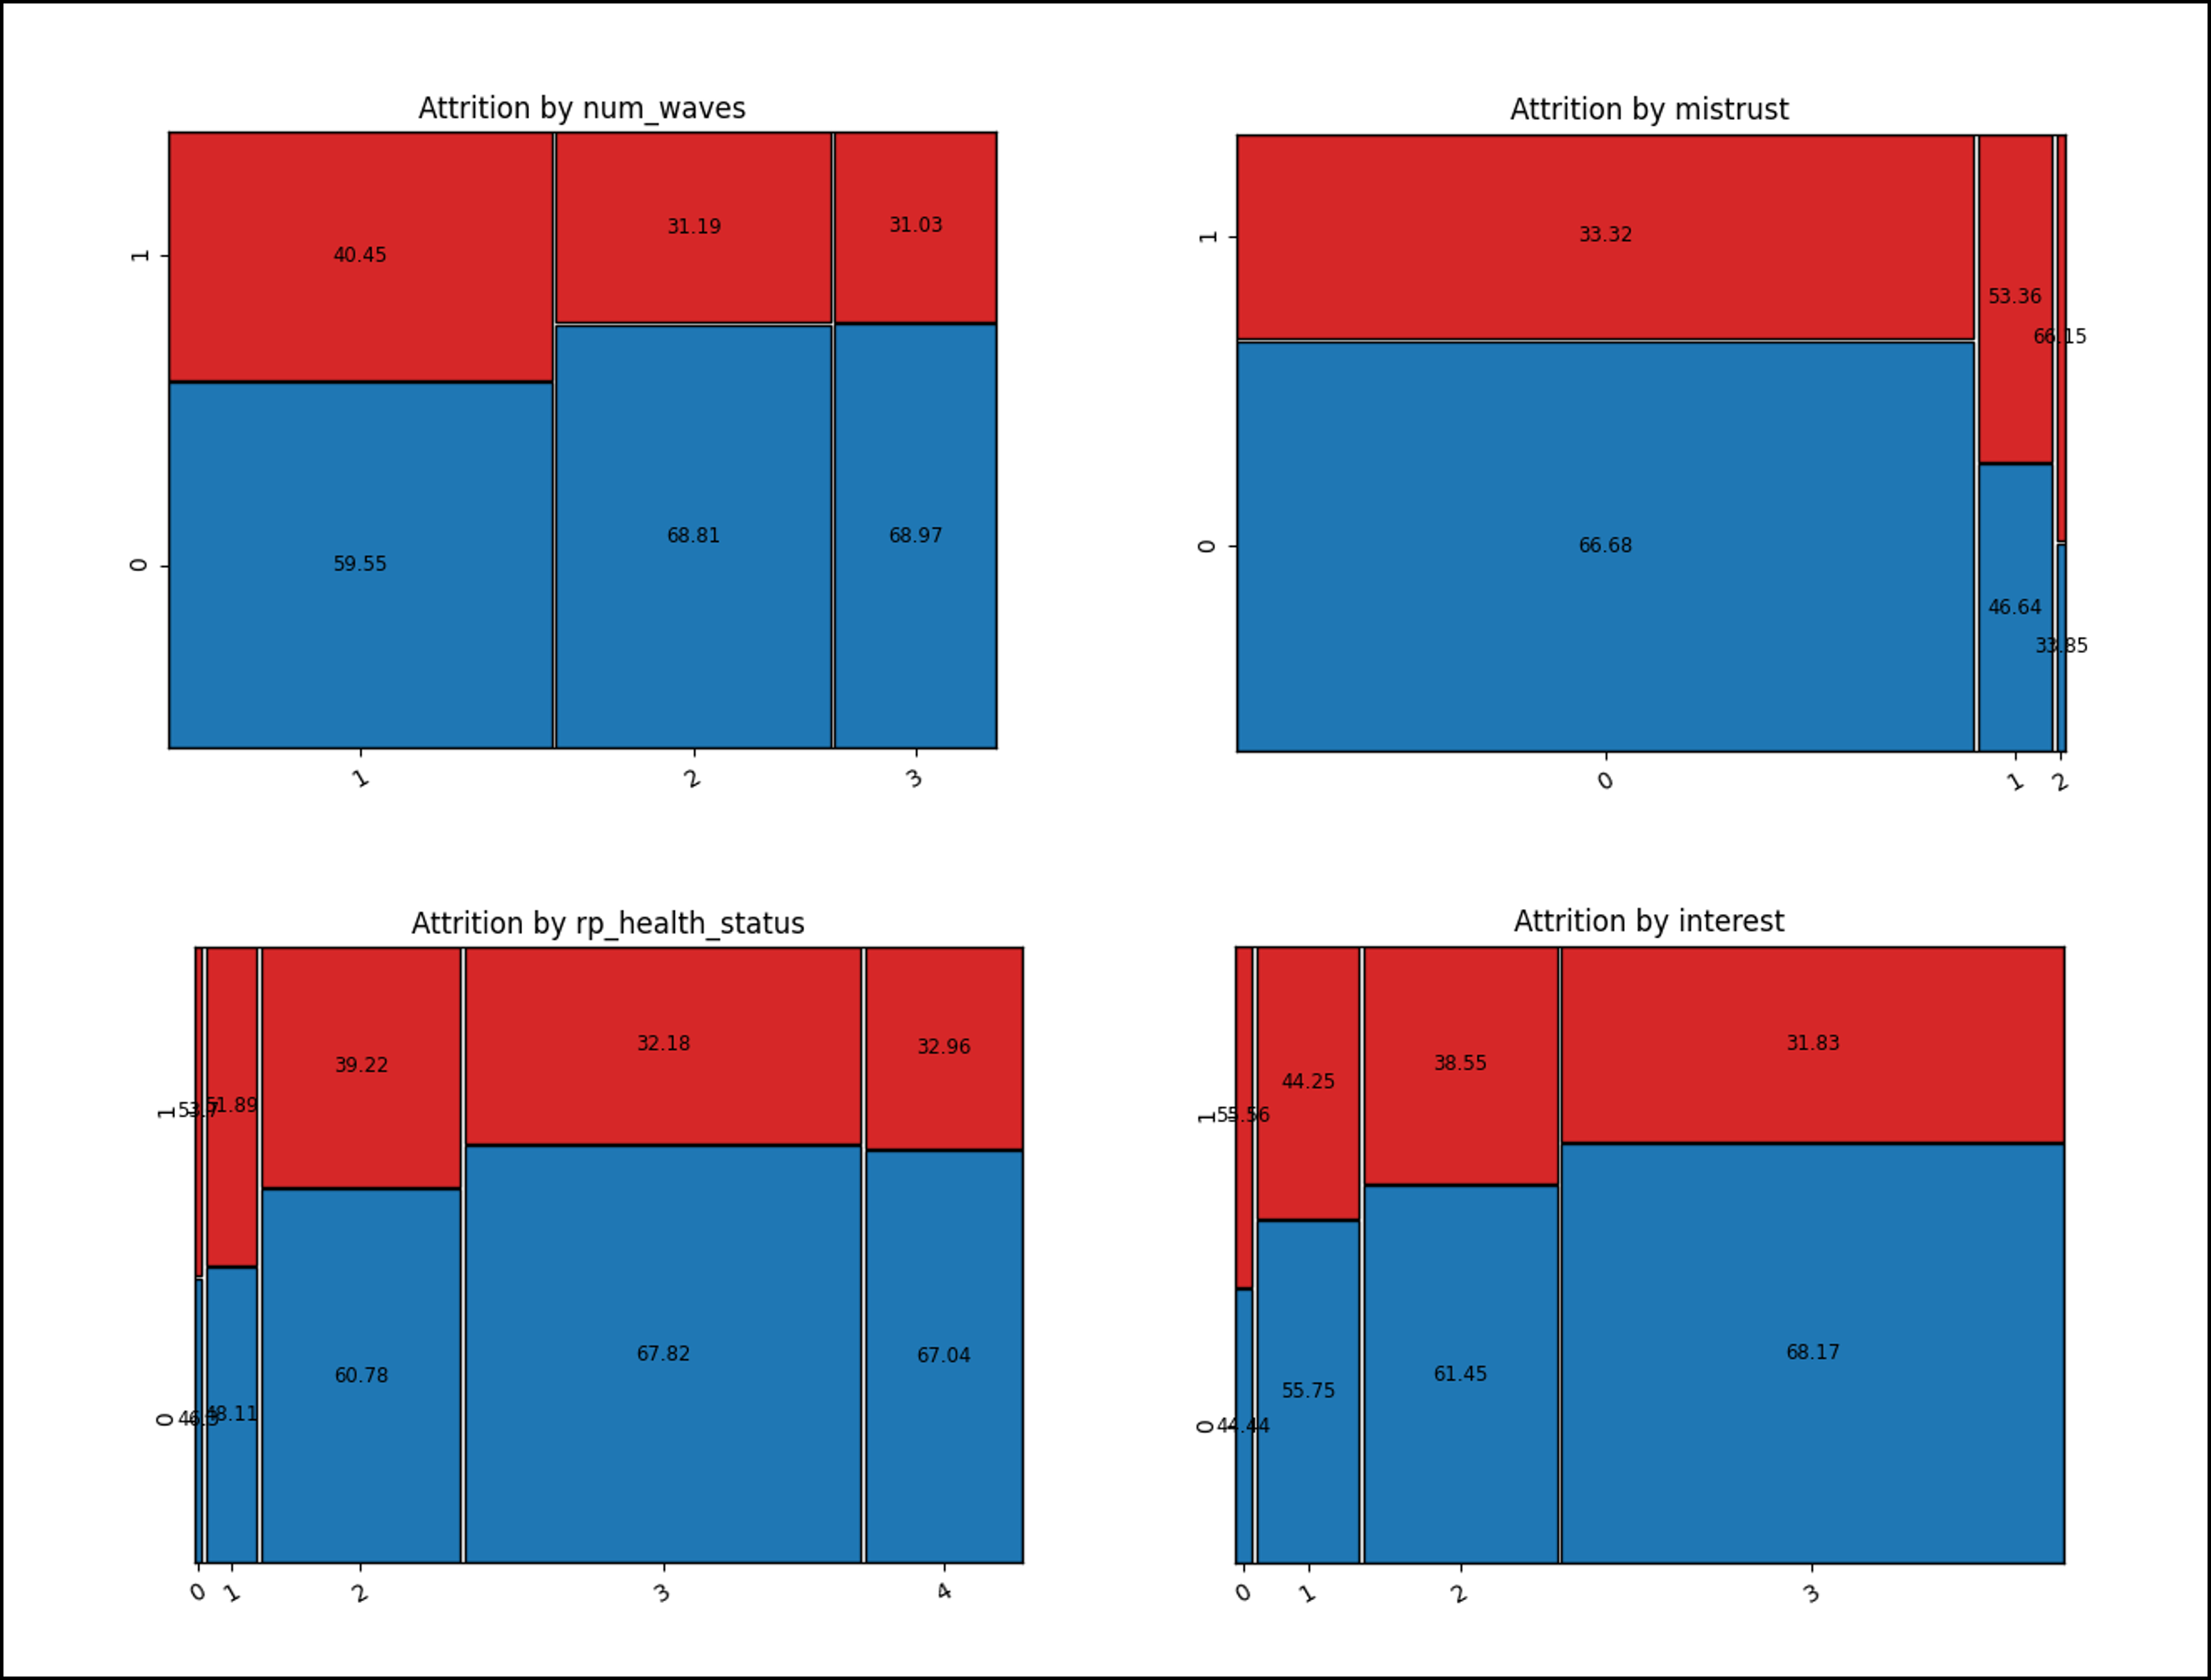
\includegraphics[width=1\textwidth]{figs/categorical.png}
	\caption{Planificación de las actividades del TFM}
	\label{fig:gantt}
\end{figure}

En la figura puede observarse que la proporción de abandono de los hogares que han participado sólo una ola es mayor que la de los que han participado en más de una. Este resultado sugiere que los hogares que llevan menos tiempo en la encuesta podrían ser más complicados de retener, y que podría ser interesante hacer un análisis enfocado en este tipo de hogares.

El segundo resultado a destacar es el del recelo mostrado por el hogar tras la entrevista. Recordemos que en la EFF se hacen preguntan que pueden considerarse delicadas, como por ejemplo si se poseen joyas, o cuál es el saldo que el hogar tiene en su cuenta corriente. Puede ser comprensible que se genere recelo. Este se mide con tres niveles: nada receloso, algo receloso y muy receloso. En el gráfico se observa que la proporción de hogares que abandonan la EFF aumenta con el nivel de recelo. Este resultado es bastante obvio, pero es muy importante resaltarlo porque a un entrevistador podría resultarle muy útil saber si el hogar con el que está a punto de contactar se mostró muy receloso después de hacer la entrevista en la ola anterior, y en su estrategia de contacto y de ganar la cooperación podría hacer más énfasis en los aspectos de la encuesta que causan más recelo.

Finalmente, los dos gráficos de la parte de inferior hacen referencia a características de la PR. En el de la izquierda se observa que la proporción de hogares que abandona la encuesta es mayor cuando menor es el nivel de salud que reporta la PR. De nuevo, esto puede parecer algo obvio porque alguien que tiene peor salud seguramenten o quiera gastar su tiempo en realizar una encuesta. Pero, de nuevo, la estrategia de contacto y de ganar la cooperación de un entrevistador puede adaptarse si ya saben que van a ver a alguien que seguramente tenga mala salud, ya sea ofreciendo hacer la entrevista en varias sesiones, o en un ambiente en el que la PR se muestre más cómoda.

Finalmente, el último gráfico muestra el nivel de interés que mostró la PR durante la entrevista durante la edición anterior. Se observa que la proporción de hogares que vuelven a participar es mayor cuanto mayor es el interés que mostraron durante la ola anterior. De nuevo, se trata de un resultado obvio. Pero, al igual que con el nivel de recelo, este podría ser un dato que podría ser muy útil para el entrevistador cuando esté preparando su estategia de contacto con el hogar.

\section{Evaluación de modelos}

Para la selección de las variables que han entrenado los modelos se han seguido X criterios. En primer lugar, se han seleccionado variables que aparecen en las implementaciones de \cite{kern2021predicting} y \cite{beste2023case} en sus modelos de machine learning. En segundo lugar, se han seleccionado variables sobre factores mencionados en la revisión de \cite{lynn2018tackling} y que han mostrado potencial para predecir la no participación de hogares panel, como por ejemplo la duración o información sobre los contactos con los hogares. En tercer lugar, se han seleccionado variables específicas que se recogen en la EFF, como la tenencia de activos, deudas o el recelo de los hogares percibido por los entrevistadores. Finalmente, tras seleccionar todas las variables anteriores, se han realizado diversos tests gráficos y estadísticos para detectar variables con correlaciones o dependencias muy altas, y se han descartado. La selección final de variables es la que aparece en el cuadro 4.2.

\begin{table}
    \centering
    \begin{tabular}{|l|p{10cm}|}
    \hline
        \textbf{Fuente de información} & \textbf{Variables} \\ \hline
        Características del hogar & Número de adultos que trabajan, Número de adultos jubilados, Propietario vivienda principal, Tamaño del hogar, Tiene otras propiedades, Tiene joyas, Posee negocios, Posee cuentas para pagos, Posee acciones que cotizan, Posee acciones que no cotizan, Posee renta fija, Posee fondos de inversión, Posee cuentas para no pagos, Posee planes de pensiones, Les deben dinero, Poseen vehículos, Percentil de renta, Percentil de riqueza Bruta, Pareja vive en el hogar, Poseen otros activos financieros, Tienen deuda, Tienen ingresos de activos, Hijos viven en el hogar, Nivel de satisfacción con la vida \\ \hline
        Características PR & Nivel de satisfacción con la vida, PR es panel, PR - nivel educativo, PR- Edad, PR - Casada, PR - Viuda, PR - Sexo, Situación laboral - Asalariado, Situación laboral - Jubilado, Situación laboral - Inactivo, PR - Estado de salud \\ \hline
        Valoraciones FI & Recelo tras la entrevista, Tipo de edificio - Unifamiliar, Barreras - portero automático, Barreras - No hay barreras, Entendimiento de las preguntas PR, Interés PR, Razones colaborar - Interesado en estos estudios, Razones para colaborar - Lo lleva el BdE, Razones para colaborar - Relevancia de la encuesta, Razones - Favor al entrevistador, Razones - Dar su opinión, Razones - Otras \\ \hline
        Paradata & PR consiente grabar la entrevista, Hogar con recontacto exitoso, Número de olas en las que se ha participado, Tamaño del municipio, Entrevista con proxy, Número de miembros del hogar que participan, Ratio estricto, Ratio amplio, Número de variables con valores missing, Duración de la entrevista \\ \hline
    \end{tabular}
    \caption{Selección de variables para entrenar los modelos de predicción}
\end{table}

El cuadro 4.3 contiene los resultados del rendimiento de los modelos entrenados sobre el conjunto de test, es decir, los resultados para predecir la no participación de los panelistas en la EFF2022. Las métricas de evaluación que se utilizan son Accuracy, Precision, Recall, F1 y ROC AUC. La métrica de referencia que utilizamos para la evaluación es la ROC AUC, que se encuentra en la parte derecha del cuadro. Esta métrica mide el rendimiento entre la tasa de falsos positivos y falsos negativos. Toma valores de 0.5 a 1, con 1 siendo un predictor perfecto, y 0.5 el que se obtendría con una estimación realizada de manera aleatoria.

\begin{table}[ht]
    \centering
    \begin{tabular}{lccccc}
    \hline
        \textbf{Modelo} & \textbf{Accuracy} & \textbf{Precision} & \textbf{Recall} & \textbf{F1} & \textbf{ROC AUC} \\ \hline
        Logit & 0,6556 & 0,3749 & 0,3573 & 0,3659 & 0,5959 \\ 
        CART & 0,6434 & 0,3338 & 0,2835 & 0,3066 & 0,5521 \\ 
        Random Forest & 0,6489 & 0,3529 & 0,3148 & 0,3328 & 0,5821 \\ 
        XGBooster & 0,6718 & 0,3772 & 0,2769 & 0,3194 & 0,5911 \\ 
        Naive Bayes & 0,6254 & 0,3504 & 0,4063 & 0,3763 & 0,5798 \\ \hline
    \end{tabular}
    \caption{Métricas de evaluación de los modelos de predicción en el conjunto de test}
\end{table}


El modelo de referencia de este estudio, el Logit, presenta una ROC AUC de 0,5959. Se considera que un valor inferior a 0,6 es un resultado malo, por lo que el modelo Logit no es un buen predictor. Con respecto a los otros modelos, observamos que el CART y el Naïve Bayes presentan valores más bajos que el Logit, de 0,5521 y 0,5798 respectivamente. El Random Forest y el XGBooster, en cambio, presentan valores de 0,5821 y 0,5911 respectivalente, que son ligeramente superiores al del modelo Logit.

De estos resultados podemos ver que los modelos de Random Forest y XGBooster mejoran al Logit de referencia. Y entre estos dos, el Random Forest presenta valores un poco más altos en Accuracy y en Precision, y el XGBooster es mejor en Recall y F1. Aun así, es necesario recalcar que el valor de ROC AUC sigue estando por debajo de 0,6, por lo que, aunque se mejore el rendimiento con respecto al modelo Logit, los resultados de los test son malos.

Estos resiltados indican que hay modelos de machine learning que mejoran en rendimiento de la predicción con respecto a un Logit. Sin embargo, las métricas señalan que el rendimiento del mejor modelo es regular. La pregunta que hay que preguntarse entonces es, ¿por qué no está funcionando bien la predicción?

Una de las causas puede ser el overfitting, es decir, que los modelos no son capaces de generalizar bien porque se han adaptado demasiado bien a los datos con los que han sido entrenados, y por tanto su rendimiento no es bueno cuando se les presenta con datos nuevos. una manera de comprobar esto es haciendo el ejercicio predicción sobre los datos de entrenamiento con estos mismos modelos, y ver cómo son esos resultados. Estos resultados pueden verse en el cuadro 4.4.

\begin{table}[ht]
    \centering
    \begin{tabular}{lccccc}
    \hline
        \textbf{Modelo} & \textbf{Accuracy} & \textbf{Precision} & \textbf{Recall} & \textbf{F1} & \textbf{ROC AUC} \\ \hline
        Logit & 0,6389 & 0,4905 & 0,4518 & 0,4704 & 0,6517 \\ 
        CART & 0,6126 & 0,4594 & 0,5178 & 0,4868 & 0,6188 \\ 
        Random Forest & 0,6596 & 0,5223 & 0,4770 & 0,4986 & 0,6726 \\ 
        XGBooster & 0,6544 & 0,5144 & 0,4675 & 0,4898 & 0,6722 \\ 
        Naive Bayes & 0,6251 & 0,4741 & 0,5178 & 0,4950 & 0,6435 \\ \hline
    \end{tabular}
    \caption{Métricas de evaluación de los modelos de predicción en el conjunto de entrenamiento}
\end{table}

Como era de esperar, los resultados de las predicciones de los modelos sobre los datos de entrenamiento son mejores que los que se observan con respecto a los datos test. En este caso, el modelo que presenta mejor rendimiento es el Random Forest, con una métrica de ROC AUC de 0,6726, ligeramente superior a la del XGBooster. El resto de métricas del Ranfom Forest también son ligeramente mejores que las del XGBooster. Sin embargo, esta métrica de ROC AUC está entre 0,6 y 0,75, que lo clasifica como un test regular.

Continuando con el Random Forest, una ventaja de los modelos basados en árboles con respecto a otros modelos es que pueden ser interpretados. En el caso del Radom Forest, es posible consultar qué variables han tenido más peso a la hora de clasificar la participación de los hogares. Aunque los resultados de la predicción del training no sean buenos, merece la pena echarle un ojo por los patrones que haya podido detectar. El cuadro 4.5 presenta las 10 variables con más importancia en el modelo de Random Forest.

\begin{table}[ht]
    \centering
    \begin{tabular}{lc}
    \hline
        \textbf{Variable} & \textbf{Importancia} \\ \hline
        PR es panel & 0,0822 \\ 
        Interés PR & 0,0790 \\ 
        Razones para colaborar - Relevancia de la encuesta & 0,0605 \\ 
        Ratio amplio & 0,0594 \\ 
        Poseen vehículos & 0,0539 \\ 
        Tienen deuda & 0,0496 \\ 
        Situación laboral - Asalariado & 0,0475 \\ 
        Razones colaborar - Interesado en estos estudios & 0,0380 \\ 
        Posee planes de pensiones & 0,0353 \\ 
        PR consiente grabar la entrevista & 0,0348 \\ \hline
    \end{tabular}
    \caption{Selección de variables para entrenar los modelos de predicción}
\end{table}

La importancia de una variable en el Random Forest mide el peso relativo que ha tenido una variable concreta a la hora de crear las ramificaciones de los diferentes árboles de decisiones que va generando el Random Forest durante su entrenamiento. En este caso de la participación en la EFF2020, las tres variables que más importancia tuvieron fueron que la PR fuera panel, que la PR mostrase interés durante la entrevista, y que el entrevitador indicase que el hogar colaboró por la relevancia de la encuesta. También es interesante destacar la variable ratio amplio, que es un indicador de la no-respuesta del hogar a la hora de facilitar cantidades monerarias\footnote{El ratio amplio se define como el cociente entre el número de preguntas en euros respondidas por el hogar, ya fuera como valor puntual o como intervalos, sobre el número total de preguntas planteadas. Cuando mayor es su valor, más información ha facilitado el hogar.}. Finalmente, otra variable que es importante para hacer la clasificación es si la PR consintió que se grabase la entrevista.
\chapter{Conclusiones y futuras líneas de trabajo}
\label{chapter:conclusiones}

En este Trabajo de Final de Master se ha intentado aplicar la implementación de \cite{beste2023case} para predecir la no participación de hogares panel en encuestas longitudinales en olas futuras al caso de la Encuesta Financiera de las Familias. Para ello, se ha usado un modelo de Regresión Logística como referencia, y se han entrenado modelos CART, Random Forest, XGBooster y Naïve Bayes. El conjunto de predictores está formado por variables que potencialmente pueden explicar la participación de un hogar en la edición siguiente de la encuesta, como por ejemplo el interés mostrado por la persona que respondió a la encuesta, el nivel de recelo que mostró durante la entrevista, su nivel de salud o si consintió que la entrevista fuese grabada.

Los modelos de Random Forest y XGBooster presentaron mejores rendimientos que el modelo de referencia Logit en todas las métricas de evaluación consideradas, pero el valor de ROC AUC del mejor de los modelos no superó el valor de 0.6, lo cual lo clasifica como un predictor malo. Para intentar aprender sobre cómo se ha hecho la predicción, se hizo el ejercicio de usar los mismos modelos para hacer la predicción con el conjunto de entrenamiento. El modelo que funcionó mejor fue el Random Forest, pero su ROC AUC no superó el valor de 0,7, que lo clasifica como un predictor regular. Al observar las variables que más importancia tuvieron durante el entrenamiento del Random Forest destabacan que la persona que contestó a la estrevista a ya formase parte del hogar desde al menos dos ediciones antes, el valor del interés que mostró también era importante, y que el entrevistador considerase que el hogar participó por la relevancia de la encuesta.

A partir de los resultados que se han visto en este proyecto, se plantean las siguientes reflexiones y los posibles pasos que se podrían dar en el futuro para este proyecto:

\begin{enumerate}
    \item La exploración de los datos sugiere que las variables seleccionadas para entrenar los modelos de predicción guardan cierta relación con la variable de attrition. Pero no son suficientes para predecir bien si un hogar panel dejará de participar en la ola siguiente. Tal y como hemos comentado al principio de este capítulo, la EFF genera una gran cantidad de variables, y se hizo un filtrado inicial basado en las implementaciones de \cite{beste2023case} y \cite{kern2021predicting}. Es posible que haya \textbf{variables que no se han incluido, y que tengan poder para predecir el attrition}. Una vía de trabajo para el futuro es \textbf{volver a revisar toda la información disponible y plantear una nueva selección de variables}. El uso de métodos de machine learning para selección de variables es una opción que se podría implementar.
    \item Las olas de la EFF seleccionadas para el estudio son las de los años 2017, 2020 y 2022 porque son las que tienen mayor cantidad de datos y también los de mayor calidad. Todos los modelos entrenados buscan utilizar datos de lo que había en 2017 para predecir algo que iba a ocurrir en 2020, que es el año en el que tuvo lugar la crisis del \textbf{Covid-19}. Y posteriormente, en el test, se utiliza información recogida durante 2020 para predecir lo ocurrido en el año 2022, cuando el mundo estaba ya superando la crisis del Covid-19. El año 2020 fue un año especial en la EFF porque seguramente mucha gente fuera más reticente a participar por el covid, lo cual afectaría a la variable target del entrenamiento). También se tuvo que cambiar la metodología de la entrevista, pasando de entrevista personal a entrevista telefónica, que afecta a la calidad de los datos (\cite{lynn2018tackling}), y por tanto a los datos de los predictores usados en el test. Ante esta problemática, se plantean dos posibles alternativas:
    \begin{enumerate}
        \item Las olas de \textbf{EFF2002 a EFF2017 son homogéneas} en lo que a metodología se refiere. Todas las entrevistas fueron personales, y no hubo una crisis como la del Covid-19. Una alternativa interesante sería crear \textbf{nuevos modelos de predicción}, pero utilizando sólo la información disponible en esas olas. Serían \textbf{menos variables} (las respuestas de los hogares y la información recogida por los entrevistadores), pero podría ser que el rendimiento fuese mejor.
        \item La EFF va a continuar realizándose en los próximos años, y con una frecuencia bienal. Se puede volver a \textbf{plantear esta misma metodología dentro unos años, utilizando sólo ediciones completadas después de 2020}, y con el beneficio de recoger toda la información que se ha estado recogiendo en las últimas ediciones y que no está disponible para antes de 2017.
    \end{enumerate}
    \item Los resultados de las predicciones sobre los datos de entrenamiento también podría explicarse por la \textbf{existencia de información no observable en el momento de hacer la predicción, y que además tenga más peso para determinar el resultado de la participación que la información recabada durante la ola anterior}. El Covid-19 es un buen ejemplo de algo que no se puede prever, pero otra cosa que también se desconoce es qué entrevistadores habrá durante la siguiente edición. En todas las ediciones hay entrevistadores nuevos, y algunos funcionan muy bien, y otros no. Tal y como comentan \cite{lynn2018tackling} y \cite{groves2006nonresponse}, el papel del entrevistador es importante para la colaboración de los hogares y la calidad de los datos. Esto puede investigarse identificando a los hogares para los que no se han hecho buenas predicciones, y analizar por un lado cómo son las características que tienen en la ola anterior, y por otro la información que se tenga sobre la ola que se intenta predecir, y comprobar si las variables que tienen más peso para explicar la participación son las de la ola corriente o las de la ola anterior.
    \item Una opción que siempre hay que considerar es un \textbf{cambio de enfoque}. Hay dos alternativas que son interesantes:
    \begin{enumerate}
        \item En la exploración de los datos vimos que los hogares que han participado sólo en una edición muestran más proporción de abandonos que los que han participado más de dos años. Una posible explicación de esto es que los hogares que han participado más de una vez están más comprometidos con el estudio, y seguramente merezca la pena \textbf{enfocar el análisis en la predicción de la participación de los paneles en su segunda ola} en vez de hacer la predicción para todos los hogares.
        \item En vez de predecir un resultado binario, de participar o no participar, se puede plantear hacer un ejercicio de \textbf{análisis de superviviencia} (survival analysis), e intentar predecir el número de ediciones en las que participará un hogar de la EFF antes de abandonar el estudio. Esta información está disponible y se podría utilizar información de todas las olas de la EFF.
    \end{enumerate}
\end{enumerate}


% bibliografia
\addcontentsline{toc}{chapter}{Bibliografía}
\bibliographystyle{apalike}
\bibliography{referencias}

\end{document}